\documentclass[xcolor=table]{beamer}
\usetheme{uic}
\usepackage{amsfonts,amsmath,oldgerm,algorithmic,algorithm}
\usepackage[font=small,labelfont=bf]{caption} % Required for specifying captions to tables and figures
\usepackage{tcolorbox}
\tcbuselibrary{listings,skins}
\usepackage{alltt,xcolor}
\usepackage{hyperref}
\usepackage{comment}
\usepackage{amsthm}
\usepackage[spanish,es-noshorthands]{babel}
\usepackage{tikz}
\usepackage{minted}


\lstdefinestyle{mystyle}{
language=C
}

\newtcblisting{mylisting}[2][]{
    arc=0pt, outer arc=0pt,
    listing only, 
    listing style=mystyle,
    title=#2,
    #1
}


\newcommand{\hrefcol}[2]{\textcolor{uihteal}{\href{#1}{#2}}}
\newcommand{\testcolor}[1]{\colorbox{#1}{\textcolor{#1}{test}}~\texttt{#1}}

% Please see Section 18.1 of Beamer User Guide for all the options \usefonttheme provides
\usefonttheme[onlymath]{serif}
% \usefonttheme{serif} % use this if you would like Serif font throughout (and not just for math)

\title{Fundamentos de Inteligencia Artificial}
\titlebackground{images/etsiinformatica3.jpeg}
% an asterisk will split the background:
% \titlebackground*{images/uic_seo.jpg}
\subtitle{Práctica 3. CSP}

\author{\href{mailto:jmmontes@uma.es}{José A. Montenegro}}
\date{\today}



\begin{document}

\newtheorem{mydef}{Definición}[section] % Añade [section] para que se reinicie en cada sección
\maketitle

% default is no footline, but page numbers are incredibly useful for the audience to ask questions later
\footlinecolor{uicblue}

%%%%%%%%%%%%%%%%%%%%%%%%%%%%%%%%%%%%%%%%%%%%%%%%%%%
%%%%%%%%%%%%%%%%%%%%%%%%%%%%%%%%%%%%%%%%%%%%%%%%%%%
%%%%%%%%%%%%%%%%%%%%%%%%%%%%%%%%%%%%%%%%%%%%%%%%%%%
%%%%%%%%%%%%%%%%%%%%%%%%%%%%%%%%%%%%%%%%%%%%%%%%%%%
%%%%%%%%%%%%%%%%%%%%%%%%%%%%%%%%%%%%%%%%%%%%%%%%%%%
%%%%%%%%%%%%%%%%%%%%%%%%%%%%%%%%%%%%%%%%%%%%%%%%%%%


%%%%%%%%%%%%%%%%%%%%%%%%%%%%%%%%%%%%%%%%%%%%%%%%%%%
%%%%%%%%%%%%%%%%%%%%%%%%%%%%%%%%%%%%%%%%%%%%%%%%%%%
%%%%%%%%%%%%%%%%%%%%%%%%%%%%%%%%%%%%%%%%%%%%%%%%%%%
%%%%%%%%%%%%%%%%%%%%%%%%%%%%%%%%%%%%%%%%%%%%%%%%%%%
%%%%%%%%%%%%%%%%%%%%%%%%%%%%%%%%%%%%%%%%%%%%%%%%%%%
%%%%%%%%%%%%%%%%%%%%%%%%%%%%%%%%%%%%%%%%%%%%%%%%%%%
%###########################################################################
% Contenidos
%###########################################################################
\small


\begin{frame}{Contenido}
\tableofcontents
\end{frame}


\section{Bibliotecas}



%%%%%%%%%%%%%%%%%%%%%%%%%%%%%%%%
\begin{frame} \frametitle{Bibliotecas} 

\begin{itemize}
    \item El libro tiene implementaciones en python que se pueden encontrar en el siguiente enlace:
\url{https://github.com/aimacode/aima-python/blob/master/index.ipynb}
Utilizaremos algunos elementos de la la biblioteca de aima.


\item En este caso contrario vamos a utilizar la librería python-constraint

\url{https://python-constraint.github.io/python-constraint/index.html}

\end{itemize}


\end{frame} 


%%%%%%%%%%%%%%%%%%%%%%%%%%%%%%%%
%%%%%%%%%%%%%%%%%%%%%%%%%%%%%%%%

\section{Ejemplo básico python-constraint}

%%%%%%%%%%%%%%%%%%%%%%%%%%%%%%%%
\begin{frame} [fragile]\frametitle{Ejemplo básico python-constraint...}  \footnotesize  

\begin{minted}{python}
from constraint import Problem, AllDifferentConstraint

# Definir el problema
problem = Problem()

# Definir las variables y sus dominios
problem.addVariable('A', [1,3,8,5])
problem.addVariable('B', [3,6,8])
problem.addVariable('C', [1,8,9])
problem.addConstraint(AllDifferentConstraint())

# Definir las restricciones
def suma_menor_que_10(a, b, c):
    return a + b + c < 10

\end{minted}
\end{frame} 

%%%%%%%%%%%%%%%%%%%%%%%%%%%%%%%%

%%%%%%%%%%%%%%%%%%%%%%%%%%%%%%%%
\begin{frame} [fragile]\frametitle{...Ejemplo básico python-constraint}  \footnotesize  

\begin{minted}{python}

problem.addConstraint(suma_menor_que_10, ('A', 'B', 'C'))
#problem.addConstraint(lambda a, b,c : a+b+c <10, ('A','B','C')) #Definición equivalente

# Resolver el problema
solutions = problem.getSolutions()

# Imprimir las soluciones encontradas
for solution in solutions:
    print(solution)
\end{minted}
\end{frame} 

\section{Estructura General Problemas}

%%%%%%%%%%%%%%%%%%%%%%%%%%%%%%%%
\begin{frame} \frametitle{Estructura General Problemas}  \footnotesize  

\begin{enumerate}
    \item Creamos el problema: \\
        \textit{problem = Problem()}
    \item Añadimos variables y sus dominios:\\ 
            \textit{problem.addVariable('A', [1,3,8,5])}
    \item Añadimos restricciones:\\ 
            \textit{problem.addConstraint(AllDifferentConstraint())}
    \item Obtenemos la solución / soluciones:\\
            \textit{solutions = problem.getSolutions()}
\end{enumerate}
\end{frame} 

%%%%%%%%%%%%%%%%%%%%%%%%%%%%%%%%
\begin{frame} [fragile]\frametitle{Algoritmos } \footnotesize  

\begin{enumerate}

\item Existen varias posibles configuraciones para aplicar el algoritmo que resuelva el CSP

\begin{minted}{python}
problem = Problem(BacktrackingSolver(forwardcheck=True)) # por defecto
problem = Problem(BacktrackingSolver(forwardcheck=False))
problem = Problem(RecursiveBacktrackingSolver())
problem = Problem(MinConflictsSolver())
\end{minted}
 
\end{enumerate}

\scriptsize
Más información: 
\url{https://python-constraint.github.io/python-constraint/reference.html#solvers}
\end{frame} 
%%%%%%%%%%%%%%%%%%%%%%%%%%%%%%%%
\begin{frame} [fragile]\frametitle{Restricciones } \footnotesize  

\begin{enumerate}

\item Definir las restricciones como función estándard:

\begin{minted}{python}
def suma_menor_que_10(a, b, c): return a + b + c < 10
problem.addConstraint(suma_menor_que_10, ('A', 'B', 'C'))
\end{minted}
 
\item  Definir las restricciones como función lambda:
\begin{minted}{python}
problem.addConstraint(lambda a, b,c : a+b+c <10, ('A','B','C')) 
problem.addConstraint(lambda a, b: abs(a - b) > 1, ("Lengua", "Inglés"))
problem.addConstraint(lambda a: a != 1 and a != 6, ("Matemáticas",))
problem.addConstraint(lambda a: a == 2 or a == 4, ("Filosofía",))

\end{minted}
\end{enumerate}

\scriptsize
Más información: 
\url{https://python-constraint.github.io/python-constraint/reference.html#constraints}
\end{frame} 



%%%%%%%%%%%%%%%%%%%%%%%%%%%%%%%%
\begin{frame} [fragile]\frametitle{Ejemplo 1- Valor 3 Variables} \footnotesize  

\begin{minted}{python}
from constraint import Problem, AllDifferentConstraint
problem = Problem()
problem.addVariable('A', [1,3,8,5])
problem.addVariable('B', [3,6,8])
problem.addVariable('C', [1,8,9])
problem.addConstraint(AllDifferentConstraint())
def suma_menor_que_10(a, b, c):
    return a + b + c < 10
problem.addConstraint(suma_menor_que_10, ('A', 'B', 'C'))
#problem.addConstraint(lambda a, b,c : a+b+c <10, ('A','B','C')) #Definición equivalente

solutions = problem.getSolutions()

for solution in solutions:
    print(solution)
\end{minted}
\end{frame} 

%%%%%%%%%%%%%%%%%%%%%%%%%%%%%%%%%
\begin{frame}  \frametitle{Ejemplo 2: Mapa de Australia} \footnotesize

\begin{figure}
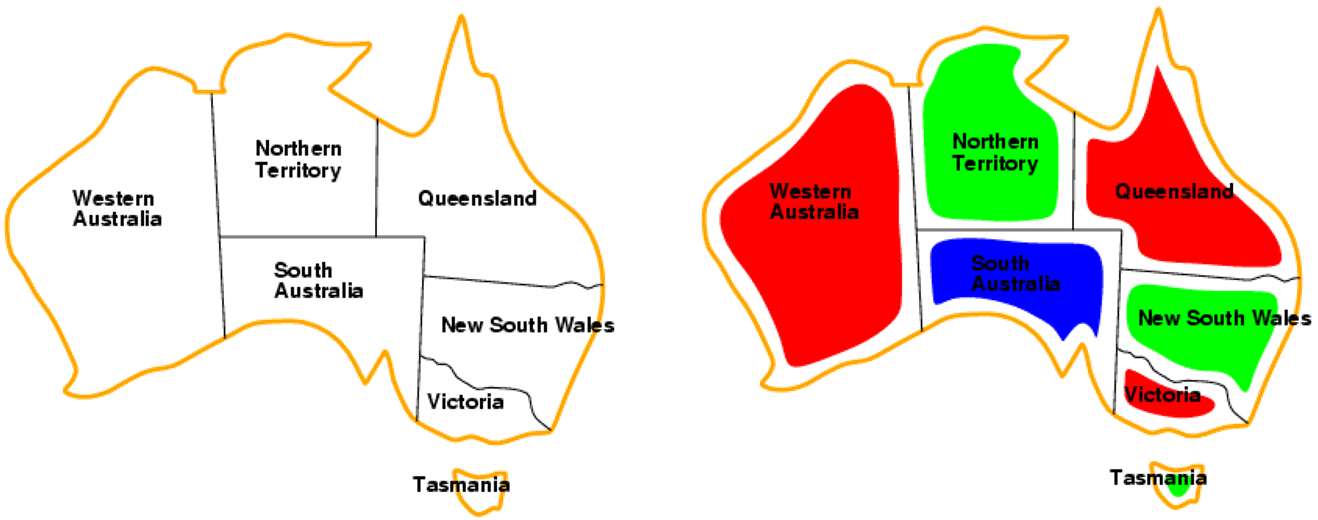
\includegraphics[scale=0.45]{./images/MapaAustralia}
\end{figure}

\begin{itemize}
\item Ejemplo de solución completa y consistente:\\
 WA = red, NT = green, Q = red, NSW = green, V = red, SA = blue, T = green

\end{itemize}

\end{frame} 
%%%%%%%%%%%%%%%%%%%%%%%%%%%%%%%%%

\begin{frame} [fragile]\frametitle{Ejemplo 2: Mapa de Australia} \footnotesize  

\begin{minted}{python}
def MapaAustralia ():    

     colors=['red','green','blue']
     
     p = Problem()  
     
     adjoins = [('SA', 'WA'), ('SA', 'NT'), ('SA', 'Q'), ('SA', 'NSW'), ('SA', 'V'),
           ('NT', 'WA'), ('NT', 'Q'), ('NSW', 'Q'), ('NSW', 'V')]  
     vars = ["WA","NT","SA","Q","NSW","V","T"]
    
     p.addVariables(vars, colors)
     
     for (v1, v2) in adjoins:         
          p.addConstraint(lambda x,y: x!=y, [v1, v2])     
     
    
\end{minted}
\end{frame} 


%%%%%%%%%%%%%%%%%%%%%%%%%%%%%%%%%

\begin{frame} [fragile]\frametitle{Ejemplo 2: Mapa de Australia} \footnotesize  

\begin{minted}{python}
     
     solution = p.getSolution()     
     
     if solution:         
          for v in vars:             
               print ("%s:%s " % (v, solution[v]),)         
               print     
     else:        print ("No solution found :-(")
\end{minted}
\end{frame} 

%%%%%%%%%%%%%%%%%%%%%%%%%%%%%%%%%

\begin{frame} [fragile]\frametitle{Ejemplo 2: Mapa de Australia} \footnotesize  

\begin{enumerate}
    \item Añadir resticciones unitarias, p.ej. SA = red p.addConstraint(lambda x: x == 'red', ['SA']) 
    \item Repetir el problema con el mapa de españa, de forma que mantenemos los mismos colores y las variables son las comunidades autónomas. Tendrá que modificar las variables y las relaciones de las comunidades colindantes.


\begin{figure}
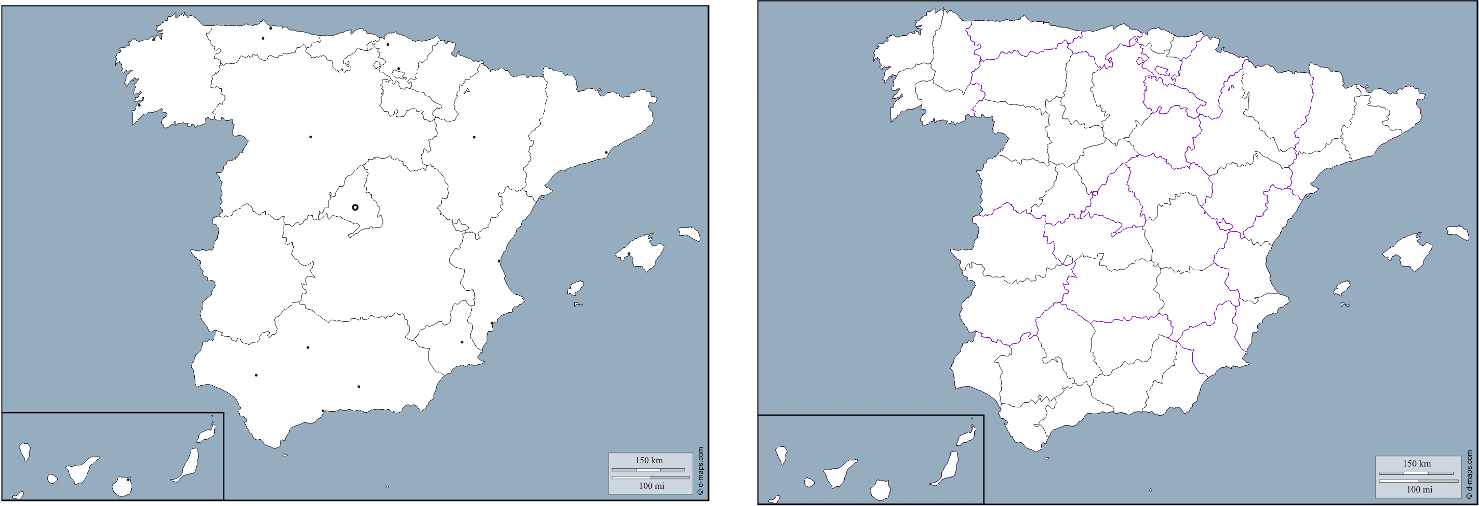
\includegraphics[scale=0.45]{./images/MapaEspanha.png}
\end{figure}
\end{enumerate}


\end{frame} 

%%%%%%%%%%%%%%%%%%%%%
\begin{frame}  \frametitle{Ejercicio 1: problemas criptoaritméticos} \footnotesize

En un acertijo criptoaritmético, cada letra representa a un dígito distinto (0-9)


\begin{columns}

\begin{column}{0.5\textwidth}
\begin{figure}

\includegraphics[scale=0.45]{./images/Cripto}
\end{figure}\end{column}

\begin{column}{0.5\textwidth}
   \begin{figure}

\includegraphics[scale=0.45]{./images/sendmoremoney}
\end{figure}

\end{column}
\end{columns}


\end{frame} 
%%%%%%%%%%%%%%%%%%%%%
\begin{frame}  \frametitle{Ejercicio 2: Diseño de un horario} \footnotesize

El director de un instituto tiene que diseñar el horario de una clase. Para simplificar
vamos a suponer que el mismo horario se aplica a todos los días. Hay seis horas, que deben rellenarse con estas asignaturas: Lengua, Inglés, Matemáticas, Física, Filosofía y Biología. Hay algunas restricciones:

\begin{itemize}
    \item Las horas de Lengua e Inglés no pueden estar adyacentes, para que los alumnos no mezcle ambos idiomas.
    \item  Las Matemáticas no deben enseñarse a primera ni a última hora, para que los estudiantes estén lo suficientemente atentos.
    \item La Física debe ir después de las Matemáticas.
    \item La Filosofía sólo se puede asignar a la segunda o a la cuarta hora.
\end{itemize}



\end{frame} 

%%%%%%%%%%%%%%%%%%%%%
\begin{frame}  \frametitle{Ejercicio 3: Sudoku} \footnotesize

Resolución del problema clásico de Sudoku.

\begin{figure}
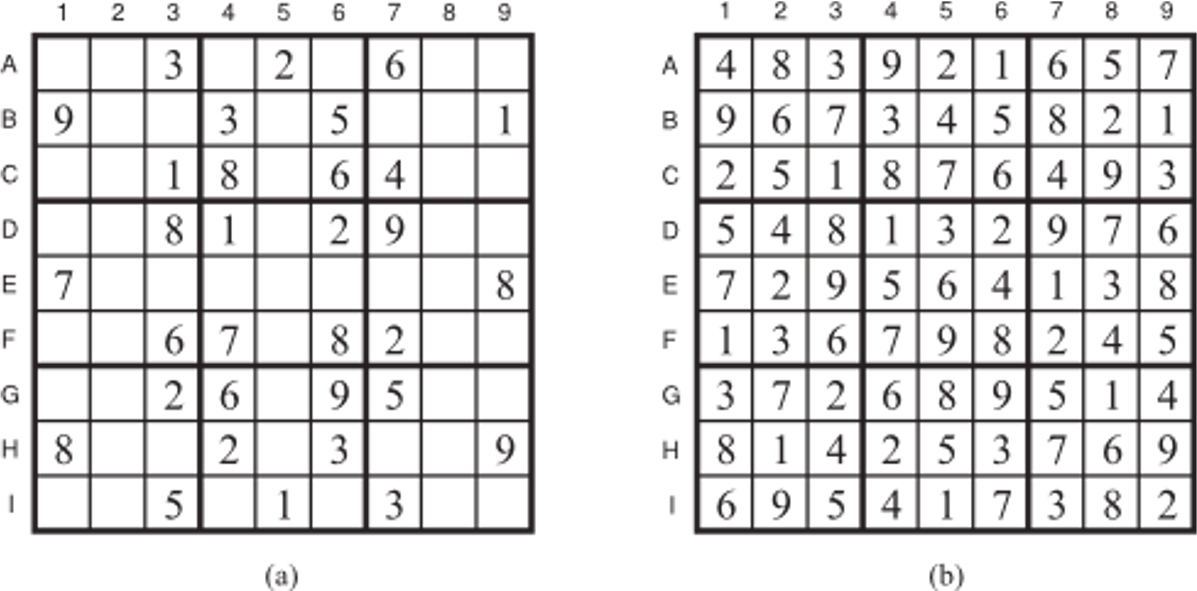
\includegraphics[scale=0.35]{./images/Sudoku}
\end{figure}

\begin{itemize}
    \item Observa la definición de las restricciones por fila, columna y región 
    \item Añada estados iniciales más díficiles y estudie como evoluciona el tiempo de resolución de los problemas.
\end{itemize}


\end{frame} 


\begin{frame} [fragile]\frametitle{Ejercicio 3: Sudoku} \footnotesize  

\begin{minted}{python}
     
    easy = [[0,9,0,7,0,0,8,6,0],
        [0,3,1,0,0,5,0,2,0],
        [8,0,6,0,0,0,0,0,0],
        [0,0,7,0,5,0,0,0,6],
        [0,0,0,3,0,7,0,0,0],
        [5,0,0,0,1,0,7,0,0],
        [0,0,0,0,0,0,1,0,9],
        [0,2,0,6,0,0,0,5,0],
        [0,5,4,0,0,8,0,7,0]]

\end{minted}
\end{frame} 

%%%%%%%%%%%%%%%%%%%%%

%%%%%%%%%%%%%%%%%%%%%
\begin{frame}  \frametitle{Ejercicio 4: Puzzle Lógico} \small

Cinco casas consecutivas tienen colores diferentes y son habitadas por hombres de diferentes nacionalidades. Cada uno tiene un animal diferente, una bebida preferida y fuma una marca determinada.\\


Además, se sabe que:\\

1. El noruego vive en la primera casa\\
2. La casa de al lado del noruego es azul\\
3. El habitante de la tercera casa bebe leche\\
4. El inglés vive en la casa roja\\

...
\end{frame} 

%%%%%%%%%%%%%%%%%%%%%
\begin{frame}  \frametitle{Ejercicio 4: Puzzle Lógico} \small

5. El habitante de la casa verde bebe café\\
6. El habitante de la casa amarilla fuma Kools\\
7. La casa blanca se encuentra justo después de la verde\\
8. El español tiene un perro\\
9. El ucraniano bebe té\\
10. El japonés fuma Cravens\\
11. El fumador de Old Golds tiene un caracol\\
12. El fumador de Gitanes bebe vino\\
13. Un vecino del fumador de Chesterfields tiene un reno\\
14. Un vecino del fumador de Kools tiene un caballo\\

Se trata de averiguar quién tiene una cebra y quién bebe agua.

\textbf{Ejercicio}: Implemente las restrciones de la 5 a la 14.

\end{frame} 


%%%%%%%%%%%%%%%%%%%%%
\begin{frame}  \frametitle{Ejercicio 5: Desafios de Creación de Plantilla (DCP) FIFA} \small

\begin{figure}
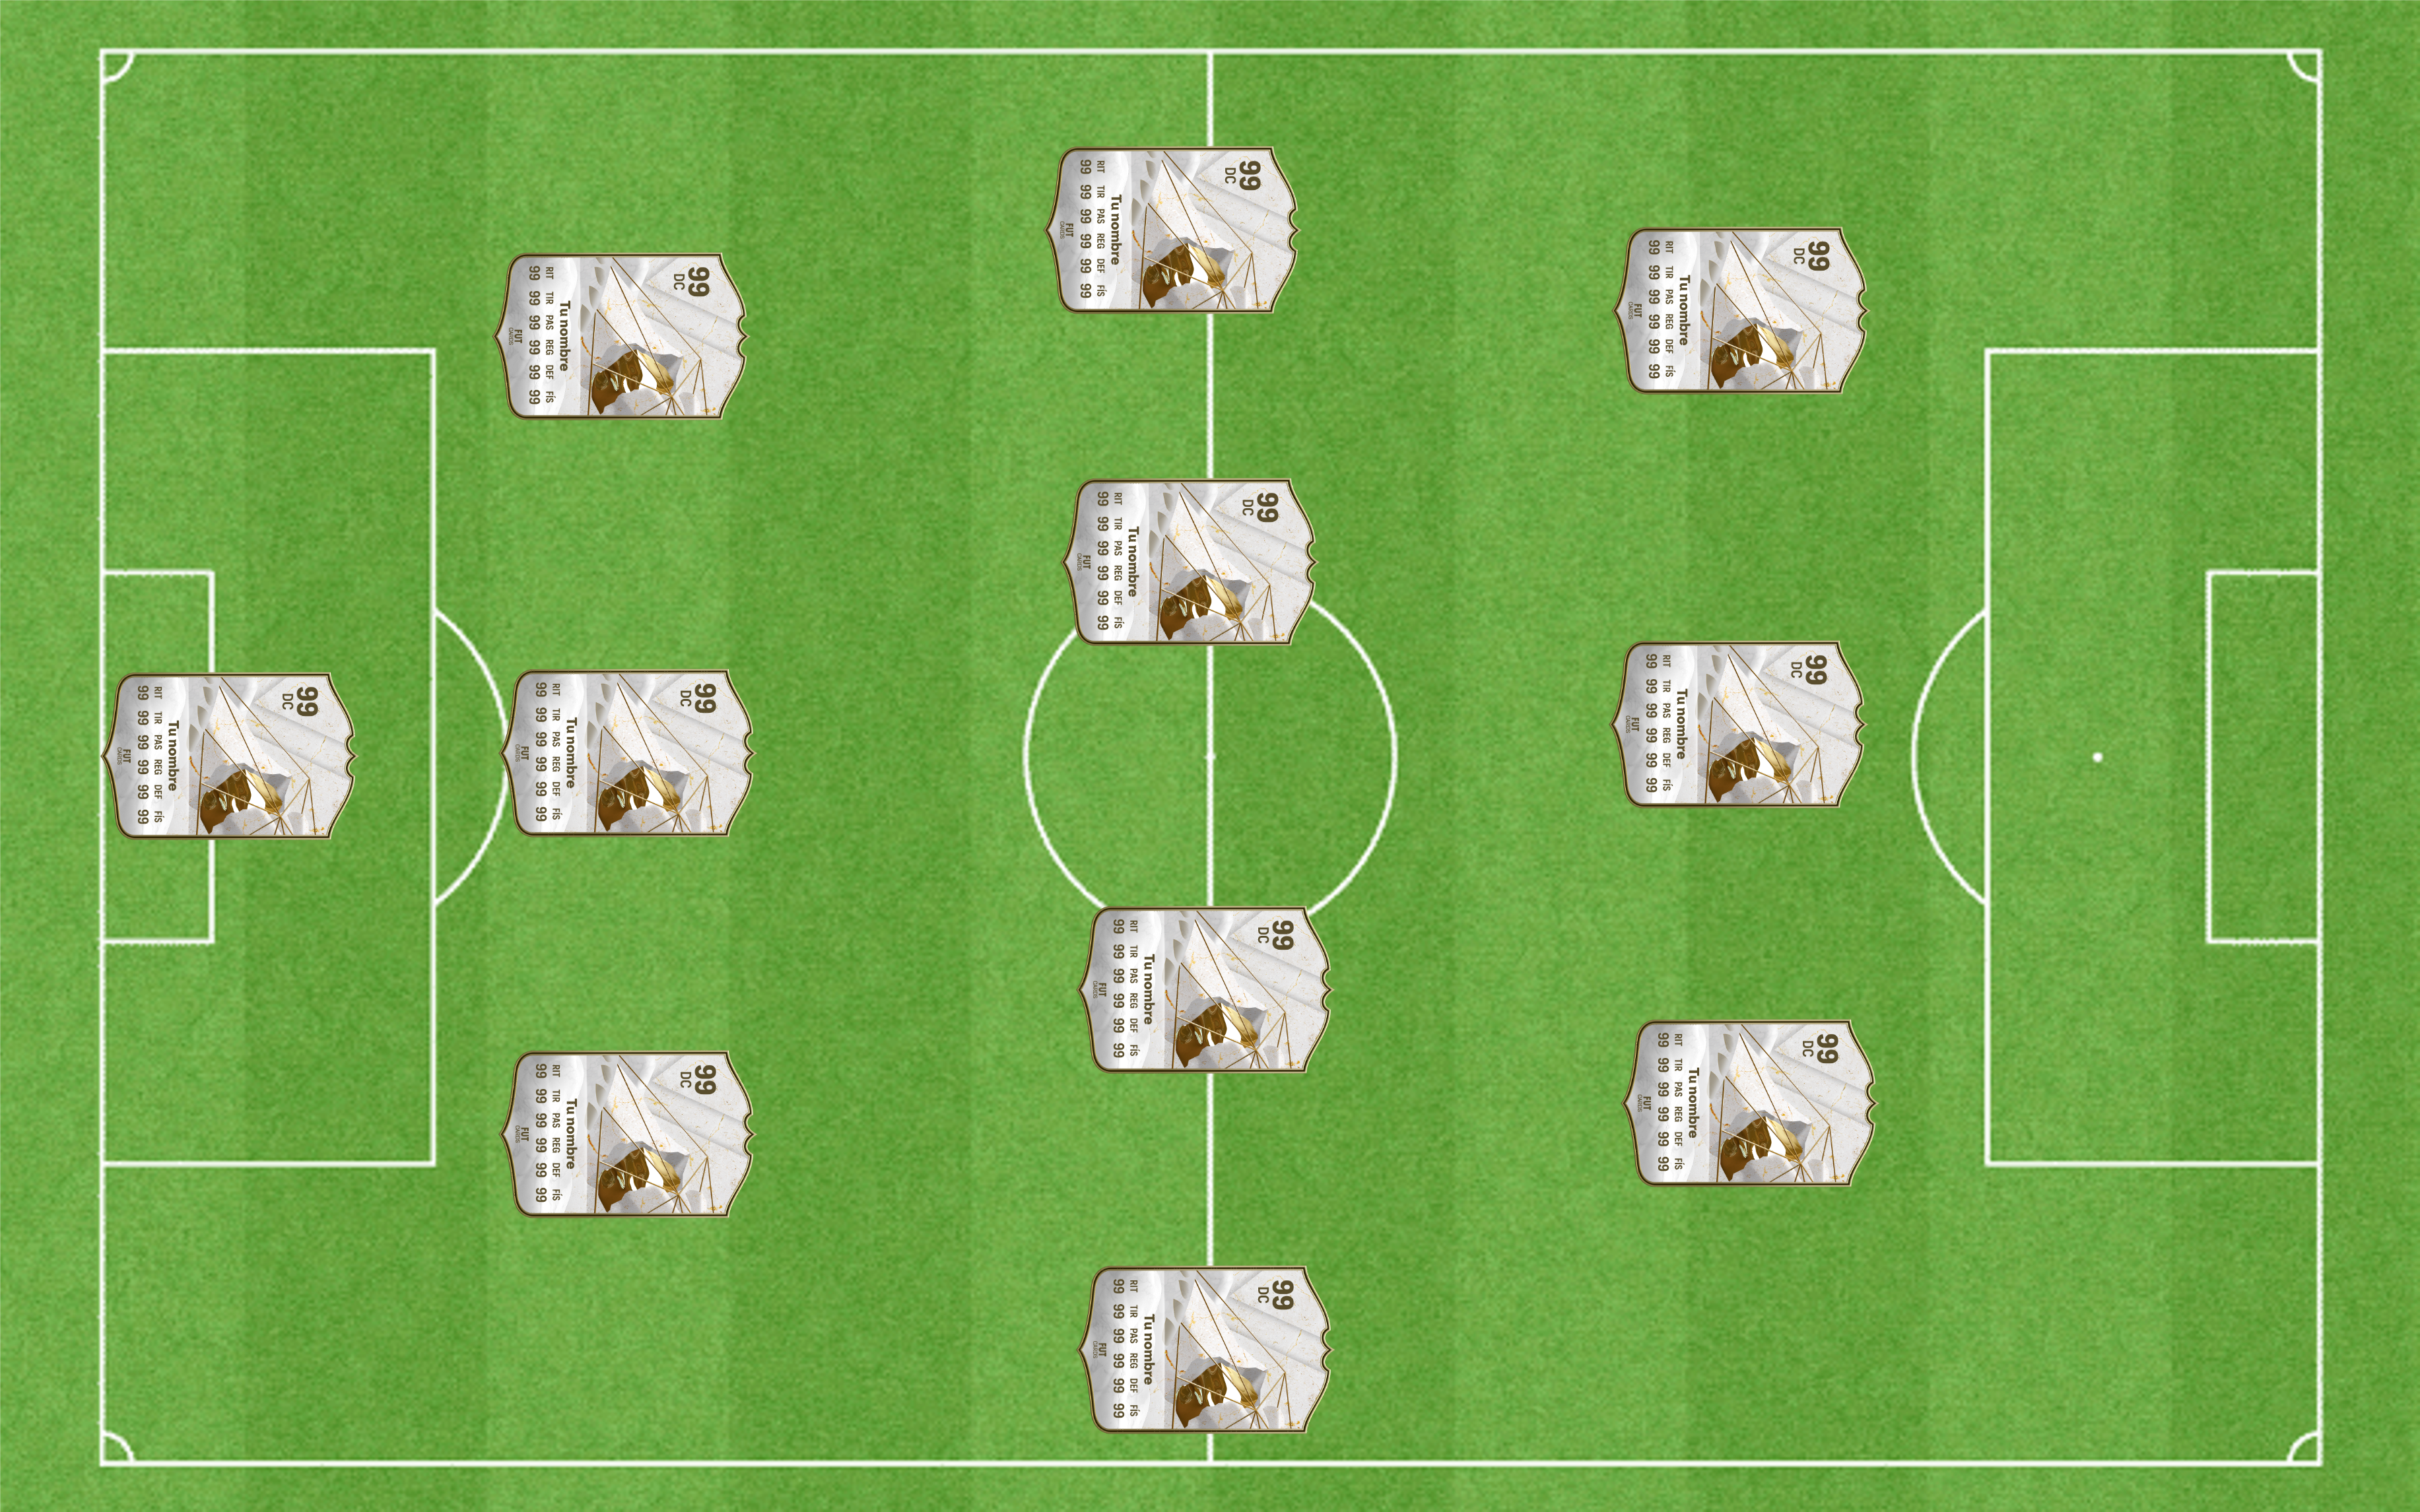
\includegraphics[scale=0.25]{./images/sbc}
\end{figure}



\end{frame} 

%%%%%%%%%%%%%%%%%%%%%
\begin{frame}  \frametitle{Ejercicio 5: Desafios de Creación de Plantilla (DCP) FIFA} \small


Vamos a simular un DCP recortado del popular juego FIFA. Para ello tenemos 5 plantillas simplificadas. En el ejemplo solo disponemos de los porteros y defensas de los equipos: Real Madrid, Barcelona, At. Madrid, Manchester City y Arsenal.\\

De cada jugador tenemos su puntuación global y su nacionalidad.\\

Tenemos que crear un equipo con la máxima puntuación:
\begin{itemize}
    \item Un portero y 3 defensas.
    \item Los jugadores elegidos tienen que ser distintos.
    \item Los jugadores deben de tener la misma nacionalidad.
\end{itemize}

\end{frame} 
%%%%%%%%%%%%%%%%%%%%%
\begin{frame}  \frametitle{Ejercicio 5: Desafios de Creación de Plantilla (DCP) FIFA} \small



\textbf{Ejercicios}:
\begin{itemize}
    \item Cambia la restricción de la nacionalidad, permiendo dos, tres y cuatro nacionalidades. Observe como se modifca el resultado.
    \item  Añada más jugadores al equipo.
    \item  Añada más clubs al problema.
\end{itemize}

\end{frame} 

%%%%%%%%%%%%%%%%%%%%%
\begin{frame}  \frametitle{Ejercicio 6: Crucigrama} \footnotesize
Crucigrama: Considera el crucigrama mostrado en la siguiente figura.

\begin{figure}
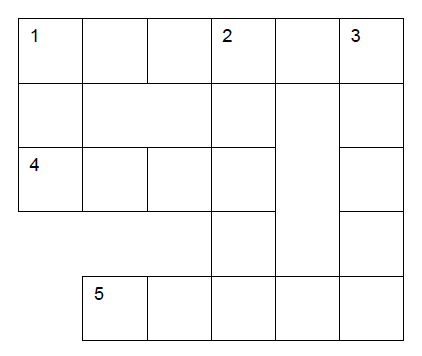
\includegraphics[scale=0.5]{./images/crucigrama}
\end{figure}
Debe resolverse con 6 palabras (1-horizontal, 1-vertical, 2-vertical, 3-vertical, 4- horizontal y 5-horizontal).

\textbf{Ejercicios}:
\begin{itemize}
    \item Añada elementos a los dominios.
\end{itemize}

\end{frame} 

%%%%%%%%%%%%%%%%%%%%%
\begin{frame}  \frametitle{Ejercicio 7: N reinas} \small
Resuelva el problema de las N-reinas

\begin{figure}
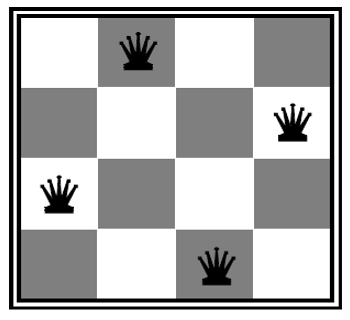
\includegraphics[scale=0.75]{./images/Nreinas}
\end{figure}


\end{frame} 

%%%%%%%%%%%%%%%%%%%%%
\begin{frame}  \frametitle{Ejercicio 8: Planificación de un proyecto} \footnotesize

Un proyecto de ingeniería se compone de varias tareas.

Cada una de ellas tiene su propia duración y sus prerrequisitos, es decir, otras tareas que deben terminarse antes de que la tarea empiece. Esta información viene dada por la siguiente tabla.

\begin{table}[]
\begin{tabular}{|c|c|c|}
\hline
\rowcolor[HTML]{C0C0C0} 
{\color[HTML]{333333} \textbf{Tarea}} & {\color[HTML]{333333} \textbf{Duración (meses)}} & {\color[HTML]{333333} \textbf{Prerrequisitos}} \\ \hline
A                                     & 3                                                & -                                              \\ \hline
B                                     & 4                                                & A                                              \\ \hline
C                                     & 2                                                & A                                              \\ \hline
D                                     & 5                                                & B, C                                           \\ \hline
E                                     & 2                                                & D                                              \\ \hline
F                                     & 2                                                & D, E                                           \\ \hline
\end{tabular}
\end{table}

Queremos saber si hay una forma de terminar el proyecto en L meses cumpliendo con los requisitos anteriores.

\end{frame} 

%%%%%%%%%%%%%%%%%%%%%%%%%%%%%%%%
%\begin{frame}  \small  
%\end{frame} 


%%%%%%%%%%%%%%%%%%%%%%%%%%%%%%%%
%\begin{frame}  \small  
%\end{frame} 


%%%%%%%%%%%%%%%%%%%%%%%%%%%%%%%%
%\begin{frame}  \small  
%\end{frame} 

%%%%%%%%%%%%%%%%%%%%%%%%%%%%%%%%%%%%%%%%%%%%%%%%%%%
%%%%%%%%%%%%%%%%%%%%%%%%%%%%%%%%%%%%%%%%%%%%%%%%%%%
%%%%%%%%%%%%%%%%%%%%%%%%%%%%%%%%%%%%%%%%%%%%%%%%%%%

%%\begin{chapter}[images/etsiinformatica4.png]{uicblue}{Introducción}
%\end{chapter}

%%%%%%%%%%%%%%%%%%%%%%%%%%%%%%%%%%%%%%%%%%%%%%%%%%%
%%%%%%%%%%%%%%%%%%%%%%%%%%%%%%%%%%%%%%%%%%%%%%%%%%%


%%%%%%%%%%%%%%%%%%%%%%%%%%%%%%%%%%%%%%%%%%%%%%%%%%%
%%%%%%%%%%%%%%%%%%%%%%%%%%%%%%%%%%%%%%%%%%%%%%%%%%%
%%%%%%%%%%%%%%%%%%%%%%%%%%%%%%%%%%%%%%%%%%%%%%%%%%%
%%%%%%%%%%%%%%%%%%%%%%%%%%%%%%%%%%%%%%%%%%%%%%%%%%%



\backmatter


\end{document}